% kapitel2.tex
\chapter{Grundlagen}

\label{chapter:kap2}

Eine der Hauptaufgaben der Statistik ist es, Systeme zu analysieren, um eine Verbindung zwischen theoretischen Aussagen und realen Beobachtungen herzustellen.
In diesem Zusammenhang ist ein System ein abstraktes Konstrukt aus verschiedenen Entitäten, die einem bestimmten Verhalten folgen und miteinander interagieren.
Betrachten wir z. B. eine Warteschlange an einem Jahrmarktsstand und das Ziel einer Studie ist es, die durchschnittliche Anzahl der Kunden am Stand zu ermitteln, dann besteht das zu beobachtende System aus dem Stand (genannt Server), einer Warteschlange und den Kunden.
In diesem Fall können die Zeit zwischen dem Eintreffen eines neuen Kunden und die Bedienzeit eines einzelnen Kunden als statistische Prozesse beschrieben werden, und die durchschnittliche Anzahl der Kunden ist ein zufällig verteilter Wert.
Solche Systeme werden durch Warteschlange-Modelle repräsentiert, die in der Statistik weit verbreitet sind und im nächsten Abschnitt kurz beschrieben werden sollen. 

Im Allgemeinen können Systeme in zwei Arten unterteilt werden, in diskrete und kontinuierliche. 
Das gerade beschriebene System ist ein diskretes System, weil sich die Anzahl der Kunden im System immer nur um einen diskreten Wert (um genau 1) ändert, wenn ein neuer Kunde eintrifft oder nachdem ein Kunde bedient wurde.
Im Gegensatz dazu wäre ein Beispiel für ein kontinuierliches System die Bewegung eines Fahrzeugs, wo eine mögliche Statistik die Durchschnittsgeschwindigkeit wäre. 
Dieser Unterschied zwischen diskreten und kontinuierlichen Systemen überträgt sich auf die Art der Verteilungsfunktion der beobachteten Statistik und beeinflusst somit die Wahl des statistischen Modells, welches das reale System so gut wie möglich darstellen soll. 
In dieser Arbeit wird nur der diskrete Fall betrachtet.
Da die Methoden jedoch keinen Gebrauch von der Art der Verteilungsfunktion machen und sich diskrete Verteilungen mit zunehmender Anzahl der diskreten Werte einer kontinuierlichen Verteilung annähern, können die Ergebnisse leicht auf den kontinuierlichen Fall übertragen werden.

Nun gibt es mehrere Möglichkeiten, das Verhalten eines Systems bei Änderung der Eingangsparameter zu untersuchen.
Averill M. Law\cite{Law} gibt einen guten Überblick zu diesem Thema, wie in Abbildung \ref{fig:sysstudy} dargestellt.
Grundsätzlich kann unterschieden werden zwischen Experimenten, die direkt am realen System durchgeführt werden und Experimenten, die an einem Modell des Systems durchgeführt werden. 
Experimente am realen System setzen voraus, dass die physikalischen Gegebenheiten des Systems nach Belieben verändert werden können.
Für das Beispiel des Jahrmarktsstands würde dies bedeuten, dass z. B. die Ankunftsrate der Kunden gesteuert werden kann, ohne die Integrität des Systems zu beeinträchtigen.
Dieses Szenario ist der Idealfall, da es Unsicherheitsfaktoren in der Studie eliminiert, wie z. B. die Wahl des statistischen Modells.
In den meisten Fällen ist das jedoch nicht möglich, da man in der Regel nur begrenzte materielle oder monetäre Ressourcen zur Verfügung hat oder das System durch die Änderung zu sehr gestört wird.
Die am häufigsten verwendete Variante ist die Simulation, bei der versucht wird, das reale System möglichst genau mathematisch abzubilden. Durch computergestützte Simulationen können so beliebig viele Daten generiert werden.

\begin{figure}[h]
	\centering
	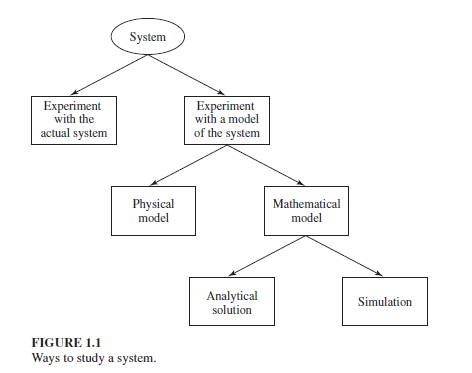
\includegraphics[]{bilder/system_study}
	\caption{Arten von Systemstudien}
  \label{fig:sysstudy}
\end{figure}

\section{Simulationsstudien}

Ein mathematisches Modell welches das reale System repräsentiert wird Simulationsmodell genannt und kann als ein Programm implementiert werden.

Dies kann beliebig komplex sein und sich so dem Verhalten des realen System annähern, allerdings ist es im Grunde eine Funktion die zu verschiedenen Eingabeparametern eine entsprechende Ausgabe berechnet.

Die Ausführung solch eines Programms zu gegebenen Eingabeparametern repräsentiert ein Experiment und wird Simulation genannt.

Eine Simulationsstudie setzt sich dementsprechend zusammen aus mehreren Simulationen zu unterschiedlichen Parameterwerten.

Ein großer Vorteil der Simulation ist, dass die durch die verschiedenen Simulationen erhobenen Stichproben per Definition unabhängig und identisch Verteilt sind, was bei Experimenten am realen System in der Regel nicht der Fall ist.

Ein einfaches Simulationsmodell welches eine Singel-Server-Warteschlange wie im Beispiel repräsentiert ist das M/M/1-Modell.

Law gibt eine gute Einführung in die Simulation solcher Modell, an der sich die Implementierung in Kapitel 4 orientiert.

Nachdem die Daten durch die Simulation erhoben wurden, wollen wir das Verhalten des Systems unter Veränderung der Parameter (etwa. der arivalrate oder servicetime) analysieren und durch eine Formel angeben.

Solch eine Formel die wiederum das Simulationsmodell vereinfacht repräsentiert ist auch ein mathematisches Modell und wird Metamodell genannt (bzw. Regressions Metamodell falls...)

Barton gibt eine gute Einführung für die Bestimmung solcher Metamodelle

Wir nehmen an, dass das Simulationsmodell das reale Modell korrekt repräsentiert, das Metamodell ist dann ... in Abhängigkeit von einem Parametervektor

Die Berechnung der Regressionsfunktion und Analyse der Methoden ist für uns primäres ziel der Simulationsstudie

Angenommen das Modell repräsentiert die Simulation und es ex. ein wahrer wert theta0, dann ist das erste Problem diesen zu bestimmen bzw zu schätzen

Die mit Abstand effektivste Methode theta in parametrischen Studien zu schätzen ist die maximum likelyhood methode, welche im nächsten abschnitt kurz vorgestellt werden soll

\subsection{M/M/1-Modell}

%%%%%%%%%%%%%%%%%%%%%%%%%%%%%%%%%%%%%%%%%%%%%%%%%%%%%
% Quellen 

Law,  A.M.  and  Kelton,  W.D.  1991.  Simulation  modeling  and analysis:

%%%%%%%%%%%%%%%%%%%%%%%%%%%%%%%%%%%%%%%%%%%%%%%%%%%%%

Ein einfaches und sehr beliebtes Simulationsmodell ist das M/M/1-Modell, welches zu der Klasse der sogenannten Warteschlangenmodelle gehört. 

Diese sind sehr simpel und leicht zu implementieren und eigenen sich daher gut, um Verfahren zu entwickeln und zu testen, welche im Anschluss für komplexere Modelle verwendet werden können.

Als anschauliches Beispiele stelle man sich vor, bei dem Modell handelt es sich um einen einzelnen Server, der alles eingehenden Aufträge nach dem "First in first out"-Prinzip (FIFO) verarbeitet.

Eingangsparameter für das Modell sind die durchschnittliche die zwischen der Ankunft eines neuen Auftrages vergeht (der Zwischenankunftszeit) und der durchschnittliche Verarbeitungszeit der Aufträge, wobei angenommen wird, dass alle Aufträge den selben Arbeitsaufwand haben.

Als Ausgangsparameter der Simulation können wir dann etwa die durchschnittliche Länge der Warteschlange oder die durchschnittliche Wartezeit messen.

Theoretische Größen, wie die Erwartungswerte und die Verteilung dieser Statistiken sind bereits für eine Vielzahl von Statistiken bekannt, sodass wir die Methoden damit vergleichen können und somit auch bewerten

Die Verteilung der Eingabeparameter sind durch die Bezeichnung gegeben, welche
auf den Mathematiker D. G. Kendall zurückgeht.

In der sogenannten "Kendall's Notation" beschreiben ersten beiden Buchstaben die Verteilung der Zwischenankunftszeiten und der Bearbeitungszeiten.

Das "M" steht dabei für "Markov" oder "memoryless" und gibt an dass es sich hier sowohl bei den Zwischenankunftszeiten, als auch bei den Bearbeitungszeiten um Poisson-Ankunfts-Prozesse mit exponentialverteilten Ankunftszeiten handelt.

Die 1 steht für die Anzahl der Server, welche zur Bearbeitung der eingehenden Aufträge zur Verfügung stehen.

Eine allgemeinere Version der M/M/1-Warteschlange ist das M/G/1-Modell, bei dem das "G" nun für "general" also eine beliebige Verteilung steht.

Diese wird im Verlauf der Arbeit ebenfalls noch einmal erwähnt.

\begin{figure}[h]
	\centering
	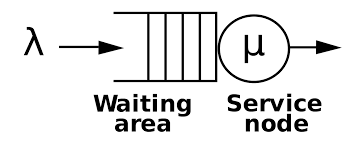
\includegraphics[width=8cm]{bilder/mm1}
	\caption{M/M/1 Warteschlangenmodell}
  \label{fig:mm1}
\end{figure}

% Verteilung der Zeitabstände zwischen Kunden
\begin{equation}
f_T(x) = \lambda e^{- \lambda t}, \quad t \geq 0
\end{equation}

% Verteilung der Zeitabstände zwischen Services
\begin{equation}
f_S(x) = \mu e^{- \mu t}, \quad t \geq 0
\end{equation}

\begin{figure}[h]
	\centering
	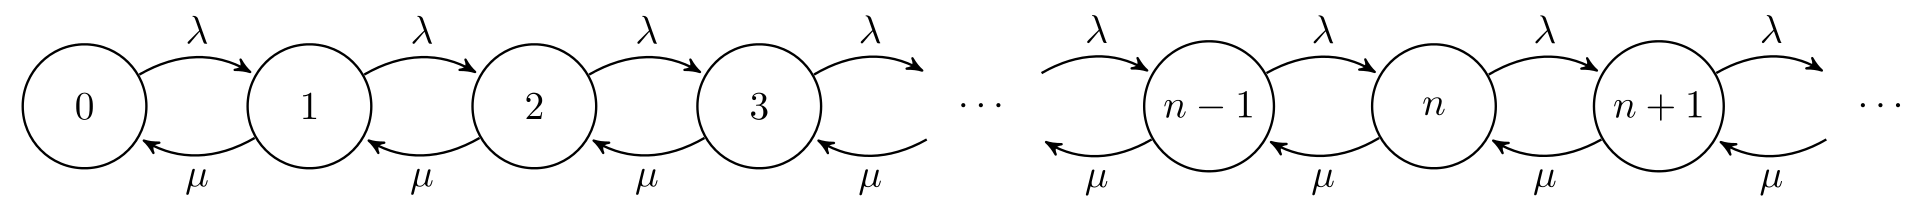
\includegraphics[width=8cm]{bilder/mm1_state}
	\caption{M/M/1 Zustandsübergangsdiagramm}
  \label{fig:mm1_state}
\end{figure}

% Verteilung für die Anzahl von Kunden im System
\begin{equation}
P_n = (1 - \rho) \rho^n
\end{equation}

% Erwartete Anzahl von Kunden im System
\begin{equation}
L = \frac{
	\rho
}{
	1 - \rho
} = \frac{
	\lambda
}{
	\mu - \lambda
}
\end{equation}

% Erwartete Wartezeit in der Queue
\begin{equation}
W_q = \frac{
	\rho
}{
	\mu - \lambda
} = \frac{
	\lambda
}{
	\mu ( \mu - \lambda )
}
\end{equation}

\section{Schätzfunktionen}

Nachdem nun durch die Simulation Daten erhoben wurden wollen wir ... ermitteln

in der Statistik dienen Schätzfunktionen dazu Schätzwerte auf Grund von empirischen Daten zu bestimmen

Bekannte Schätzfunktionen sind ... für Mittelwert und Varianz

Mittelwert uns so normalverteilt

Schätzfunktionen werden durch die Art der Schätzmethode beeinflusst, dabei sind mögliche Fehlerquellen

Eine in der Linearen Regression häufig verwendete Methode ist die Methode der kleinsten Quadrate 

Die mit Abstand effektivste Schätzmethode ist die Maximum-Likelihood-Methode, welche als Grundlage für die Konfidenzbänder dienen wird und im folgenden kurz vorgestellt werden soll

% Regressionsfunktion
\begin{equation}
y_i = \eta(x_i, \theta)+ \epsilon_i, \quad i=1,2,...,n
\end{equation}

% Verteilung der Residuen
\begin{equation}
\epsilon \sim N(0, \sigma^2)
\end{equation}

% Erwartungswert der Daten soll die Regression sein
\begin{equation}
E(y | x) = \eta(x, \theta)
\end{equation}

% Schätzer
\begin{equation}
\hat{y} = \eta(x, \hat{\theta})
\end{equation}

% Kleinsten Quadrate
\begin{equation}
\underset{\theta \in \mathcal{R}}{\arg\min} \sum_{i=1}^n \left[ \eta(x_i,\theta) - y_i \right]^2
\end{equation}

% M estimator
\begin{equation}
\sum_{i=1}^n \psi(y_i, \theta) = 0
\end{equation}

\subsection{Maximum-Likelihood-Methode}

Im Fall der Normalverteilung ist der Mittelwert genau der MLE.

Im Fall der Normalverteilung sieht man leicht, dass die Likelihood-Funktion genau dann minimal ist, wenn auch der Kleinste-Quadrate-Schätzer minimal ist

% Likelihood
\begin{equation}
\mathit{Lik}(\theta, y) = \prod_{i=1}^n f(y_i, \theta)
\end{equation}

% log Likelihood
\begin{equation}
L(\theta, y) = \log \prod_{i=1}^n f(y_i, \theta) = \sum_{i=1}^n \log f(y_i, \theta)
\end{equation}

\begin{equation}
\frac{\partial}{\partial \theta} L(\theta, y) = \sum_{i=1}^n \frac{\partial}{\partial \theta} \log f(y_i, \theta) = 0
\end{equation}

\begin{equation}
\psi = \frac{ -f }{ f }
\end{equation}

\begin{equation}
\mathrm{Var}(\theta) = \left[ I(\theta) \right]^{-1}
\end{equation}

\begin{equation}
I(\theta) = E \left(- \frac{\partial^2}{\partial \theta^2} L(\theta, y) \right) 
\end{equation}

\begin{equation}
\mathrm{Var}(\hat{\theta}) \approx \left[ \left. - \frac{\partial^2}{\partial \theta^2} L(\theta, y) \right|_{\theta = \hat{\theta}} \right]^{-1}
\end{equation}

\section{Konfidenzintervalle}

Ein $(1- \alpha)\%$ Konfidenzintevall ist direkt durch das obere und untere $z_{\alpha / 2}$ Quantil der angepassten Normalverteilung gegeben

In manchen fällen wo die Normalverteilung nicht vorausgesetzt werden kann bietet sich das Bootstrap an welches im nächsten Abschnitt vorgestellt wird

% Erwartete Wartezeit in der Queue für allgemeinere M/G/1 Systeme
\begin{equation}
W_q = \frac{
	\lambda \left[ \mathrm{Var}(S) + (E(S))^2 \right]
}{
	2 (1 - \lambda E(S)) 
}
\end{equation}

\section{Resampling Verfahren}
Zur Analyse empirischer Studien werden Resampling-Methoden gegenüber den Standardverfahren immer beliebter.

Sind sehr vielseitig einsetzbar und lösen Probleme der analytischen Ansätze.

Ermöglichen aussagekräftige Aussagen über eine Datenmenge zu erhalten ohne Annahmen über die Herkunft der Daten zu treffen.

... Zeigen, dass Resampling Methoden erstaunlich gute Ergebnisse liefern.

Wie der Begriff Resampling vermuten lässt ist die grundlegende Idee dieser Verfahren ist, wiederholt Stichproben aus einer gegebene Stichprobe zu ziehen.

Ein Problem empirischer Studien ist nämlich häufig, dass Stichprobenziehungen aufwendig und teuer sind.

Daher stehen für die Analyse oft nur wenige Stichproben zur Verfügung und man muss Annahmen über die Verteilung der Daten treffen

Resampling Verfahren umgehen dieses Problem, indem die gegebene Stichprobe als Approximation für die Grundgesamtheit verstanden wird und beliebig viele Stichproben durch erneute Stichprobenziehung erhalten werden.

Da die empirische Verteilungsfunktion der gegeben Stichprobe sich mit steigender Sample-Größe nach Monte-Carlo-Approximation der wahren Verteilung der Grundgesamtheit annähert, sind die resampletend Stichproben ebenfalls nach Monte-Carlo-Approximation eine Schätzung für die Verteilung der Grundgesamtheit

... Zeigen dass solche Resampling Verfahren exakt sind

Ein Resampling-Verfahren, welches zur Abschätzung des zufälligen Fehlers der Schätzmethode und etwaige Verzerrung der Stichprobe (Bias) zu bestimmen ist z. B. die Jackknife-Methode.

Bei der auch delete-1 Jackknife genannten Methode werden aus einer ursprünglichen Stichprobe $x_1, ..., x_n$ durch weglassen jeweils eines Wertes $n$ neue Samples gezogen. 

Der Mittelwert der Jackknife Stichprobe ist dann gegeben durch 

\begin{equation}
\hat{\theta}_{(*)} = \frac{1}{n} \sum_{i = 1}^{n} \hat{\theta}_{(i)}
\quad\text{wobei}\quad
\hat{\theta}_{(i)} = \frac{1}{n-1} \sum_{j \neq i} x_j
\end{equation}

Sei $\hat{\theta}$ der Mittelwert der ursprüngliche Stichprobe, dann kann die Varianz des Schätzer und der Bias-Wert abgeschätzt werden durch

\begin{equation}
\mathrm{Var}(x) = \frac{n-1}{n} \sum_{i=1}^{n} \left( \hat{\theta}_{(*)} - \hat{\theta}_{(i)} \right)^2
\quad\text{und}\quad
B = (n-1) (\hat{\theta}_{(*)} - \hat{\theta})
\end{equation}

Es sei angemerkt, dass hier anstelle des arithmetischen Mittelwerts auch eine beliebige andere Statistik durch das Verfahren geschätzt werden kann.

Die mit Abstand effektivste Methode ist die MLE, welche ... besprochen wird

\subsection{Bootstrap}
Das wahrscheinlich bekannteste und heutzutage wichtigste Resampling-Verfahren ist das von B. Efron 1977 eingeführte Bootstrap-Verfahren.

Es wurde als Verallgemeinerung der Jackknife-Methode entwickelt und wird dazu verwendet die theoretische Verteilungsfunktion einer Zufallsvariable durch die Empirische Verteilungsfunktion der Stichprobe zu schätzen.

Hier wird durch das Resampling die Größe der Stichprobe sozusagen künstlich vergrößert, sodass statistische Tests angewendet werden können, ohne 

Im Gegensatz zum Jackknife-Verfahren werden beim Bootstrap $B$ Stichproben der Größe $n$ aus der ursprünglichen Stichprobe mit zurücklegen gezogen.



Bootstrap ist ein sehr vielseitig einsetzbares Verfahren

wurde zum ersten mal von B. Efron 1997 erwähnt als allgemeinere Version der Jackknife-Methode

\section{Konfidenzbänder}

\section{GoF-Tests}

\subsection{Chi-Quadrat Test}

\subsection{Kolmogorov-Smirnov Test}

\begin{equation}
D = \underset{y_i}{\sup} \{ F_n(y_i) - F(y_i, \theta) \}
\end{equation}

\subsection{Anderson-Darling Test}

\begin{equation}
A^2 = -n - \sum_{i=1}^n \frac{2 i - 1}{n} \left[ \log F(y_i, \hat{\theta}) + \log( 1 - F(y_{n+1-i}, \hat{\theta})) \right]
\end{equation}

\section{Coverage Error}























